\documentclass[xcolor=x11names,dvipsnames,aspectratio=169]{beamer}
\usepackage{graphicx}
\usepackage{tikz}
\usepackage{textcomp}
\usepackage[absolute,overlay]{textpos}
\usepackage[normalem]{ulem}

\setbeamercovered{transparent}

\usetikzlibrary{positioning,arrows,snakes}
\tikzset{set/.style={draw,circle,inner sep=0pt,align=center}}
\tikzset{brace/.style={decorate, decoration={brace}},
  brace mirrored/.style={decorate, decoration={brace,mirror}}}
	\pgfdeclarelayer{background}
	\pgfsetlayers{background,main}

\usetheme{Dart}

\title{\huge DoHoT or Donion aka ``DoHoT 2 Handle''}
\subtitle{Performance of Anonymous DNS Queries}
\author{\small Jonathan, Tom, Tor, Alfred}
\date{\today}

\setcounter{showSlideNumbers}{1}

\begin{document}
    \setcounter{showProgressBar}{0}
	\setcounter{showSlideNumbers}{0}

	\frame{\titlepage}

	\setcounter{framenumber}{0}
	\setcounter{showProgressBar}{1}
	\setcounter{showSlideNumbers}{1}

    \begin{frame}{Introduction}
        Anonymous Queries
        \begin{itemize}
            \item Proxy between Client and Resolver
            \begin{itemize}
                \item Oblivious DNS
                \item Oblivious DNS-over-HTTPS (ODoH)
                \item DNS-over-HTTPS-over-Tor (DoHoT)
            \end{itemize}
        \end{itemize}
        \pause
        \vspace{1em}
        Goal: change configurations and compare performance
        \begin{itemize}
            \item Identify parameters
            \item Create containers for protocols
            \item Measure latency: \texttt{DNSHACKATHON-\{random\}.se}
        \end{itemize}
    \end{frame}

    \begin{frame}{Protocols}
        \textbf{Default DoHoT:}
        Client $\rightarrow$
        Entry $\rightarrow$
        Middle $\rightarrow$
        Exit $\rightarrow$
        DoH Resolver

        \pause
        \vspace{1em}
        \textbf{Idea 1:}
        Client $\rightarrow$
        Nearby Entry $\rightarrow$
        Nearby Exit $\rightarrow$
        DoH/DoT Resolver

        \pause
        \vspace{1em}
        \textbf{Idea 2:}
        Client $\rightarrow$
        Nearby Entry $\rightarrow$
        Nearby Exit Resolver

        \pause
        \vspace{2em}
        \begin{columns}
            \begin{column}{.5\textwidth}
                \begin{itemize}
                    \item Normal DNS (Do53)
                    \item DNS-over-HTTPS (DoH)
                    \item DNS-over-TLS (DoT)
                \end{itemize}
            \end{column}
            \pause
            \begin{column}{.5\textwidth}
                \begin{itemize}
                    \item \sout{DNS-over-Tor (DoTor)}
                    \item DNS-over-Tor (DoTor)
                    \item DoH-over-Tor (DoHoT)
                    \item DoT-over-Tor (DoToT)
                \end{itemize}
            \end{column}
        \end{columns}
    \end{frame}

    \begin{frame}{Measurement}
        \begin{columns}
            \begin{column}{.5\textwidth}
                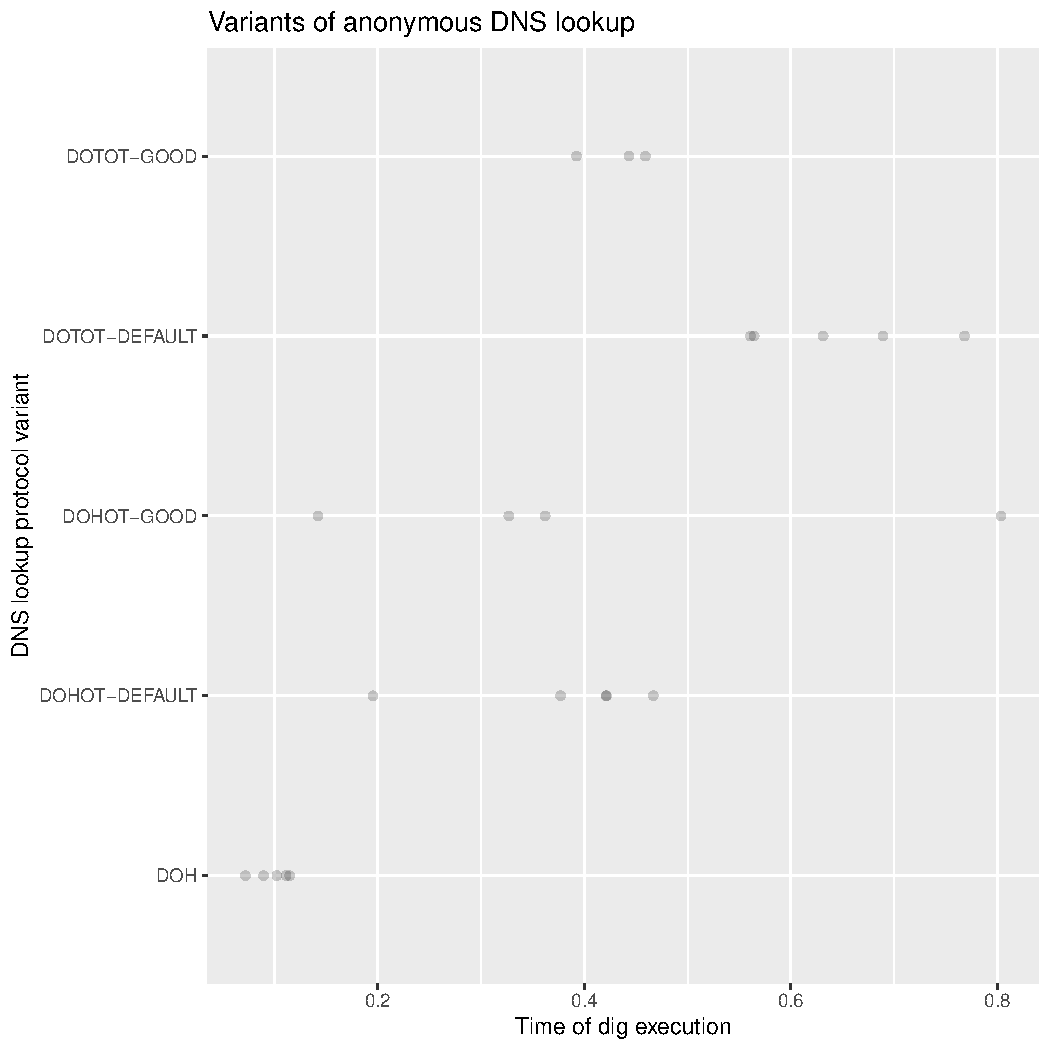
\includegraphics[width=\textwidth]{img/p1.pdf}
            \end{column}
            \begin{column}{.5\textwidth}
                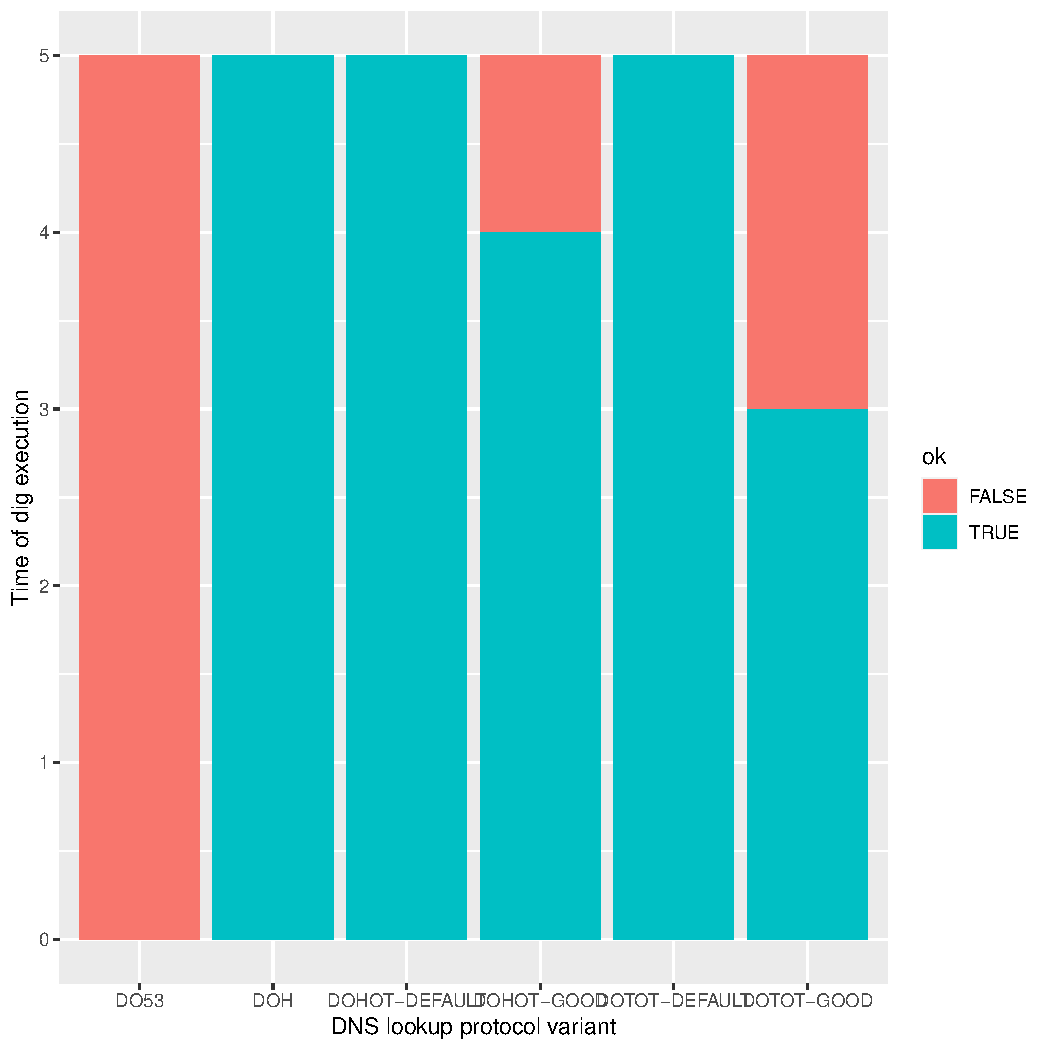
\includegraphics[width=\textwidth]{img/p2.pdf}
            \end{column}
        \end{columns}
    \end{frame}

    \begin{frame}{Artifacts}
        \url{https://github.com/DNS-Hackathon/DoHot-or-Donion}
        \begin{itemize}
            \item Docker Containers for Protocols
            \item Performance Measurement Interface
        \end{itemize}
    \end{frame}

\end{document}
